\section{results}\label{sect:result}
In this section, we are going to show the results achieved by the proposed architecture in terms of normalized mean error (NME).
Table~\ref{table:results} shows the NME compared to other approaches. As you can see, our model is able to achieve results comparable with the state-of-the-art by achieving an NME of $4.26$. Compared to the best approach our architecture falls behind only of $1.13$. 

Next, we present two samples from the test set (see Fig.~\ref{fig:pred1} and ~\ref{fig:pred2}). As you can see, our model is capable of obtaining qualitative landmarks even with fairly complex expressions. 

\begin{table}\centering
    \begin{tabular}{lc}
        \toprule
        model & NME(\%) \\\midrule
        3DDE\cite{Valle19} & 3.13 \\
        CNNCRF\cite{Chen19} & 3.30 \\
        Adaloss\cite{Teixeira19} & 3.31 \\
        SAN-GT\cite{Dong18} & 3.98 \\
        ours & 4.26 \\
        CFSS\cite{Zhu16} & 5.76 \\
        \bottomrule
    \end{tabular}
    \caption{Results from various approaches for the same task \textit{facial landmarks detection}}
    \label{table:results}
\end{table}


\begin{figure}
    \begin{subfigure}{.61\textwidth}
        \centering
        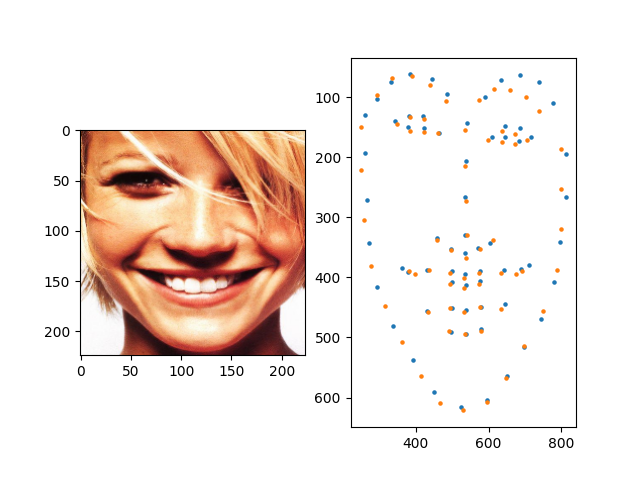
\includegraphics[width=.8\linewidth]{figs/prediction1.png}
        \subcaption{Example of prediction using our approach}
        \label{fig:pred1}
    \end{subfigure}
    \begin{subfigure}{.5\textwidth}
        \centering
        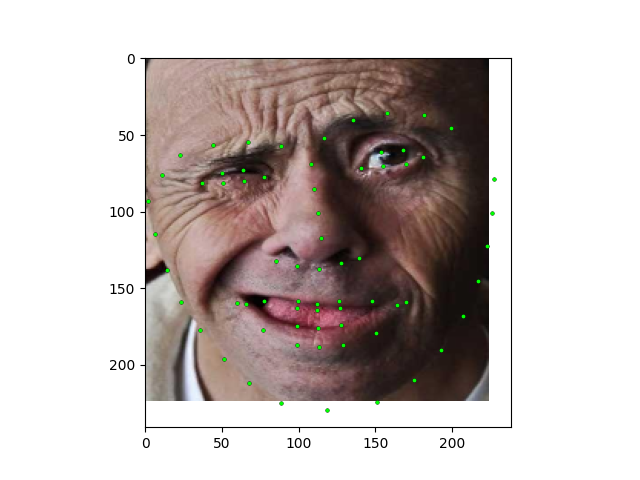
\includegraphics[width=.9\linewidth]{figs/prediction2.png}
        \subcaption{Second example of prediction using our approach}
        \label{fig:pred2}
    \end{subfigure}
    \caption{examples of predictions from the test set.}
    \label{figs:preds}
\end{figure}



